\documentclass[12pt,a4paper]{article}

% Packages
\usepackage[margin=2.5cm]{geometry}
\usepackage{graphicx}
\usepackage{hyperref}
\usepackage{listings}
\usepackage{xcolor}
\usepackage{booktabs}
\usepackage{fancyhdr}
\usepackage{float}

% Hyperlink style
\hypersetup{
    colorlinks=true,
    linkcolor=blue!60!black,
    urlcolor=blue!70!black,
}

% Code listing style
\lstset{
    basicstyle=\ttfamily\small,
    backgroundcolor=\color{gray!8},
    frame=single,
    rulecolor=\color{gray!30},
    breaklines=true,
    columns=fullflexible,
    keepspaces=true,
    showstringspaces=false,
}

% Header/Footer
\pagestyle{fancy}
\fancyhf{}
\fancyhead[L]{\small React Native Messages Directory}
\fancyhead[R]{\small \thepage}
\renewcommand{\headrulewidth}{0.4pt}

% Document info
\title{\textbf{React Native Messages Directory}\\[0.5em]\large Technical Documentation}
\author{Yao Zhang}
\date{May 1, 2026}

\begin{document}

\maketitle
\thispagestyle{empty}

\vspace{1cm}
\tableofcontents
\newpage

% ============================================================
\section{Project Overview}

This project is a React Native message directory application built with Expo and TypeScript. The app displays 6 message categories (You, Home, Love, Family, Friends, School). Tapping any category shows the stored messages for that directory. Users can also send new messages within each category.

% ============================================================
\section{Tech Stack}

\begin{itemize}
    \item React Native (Expo SDK 54)
    \item TypeScript
    \item React Navigation (Native Stack)
    \item Expo Vector Icons
\end{itemize}

% ============================================================
\section{Project Structure}

\begin{table}[H]
\centering
\begin{tabular}{@{}ll@{}}
\toprule
\textbf{File / Directory} & \textbf{Description} \\
\midrule
\texttt{App.tsx} & App entry with navigation stack \\
\texttt{index.ts} & Expo entry point \\
\texttt{src/data/messages.ts} & Category and message data \\
\texttt{src/screens/HomeScreen.tsx} & Home screen with category grid \\
\texttt{src/screens/MessagesScreen.tsx} & Messages list with send functionality \\
\texttt{package.json} & Dependencies \\
\texttt{tsconfig.json} & TypeScript configuration \\
\bottomrule
\end{tabular}
\caption{Project file structure}
\end{table}

% ============================================================
\section{Prerequisites}

\begin{itemize}
    \item Node.js (v18+)
    \item npm
    \item Expo CLI
    \item Android Studio (for Android Emulator) or Xcode (for iOS Simulator)
\end{itemize}

% ============================================================
\section{Installation and Setup}

\subsection{Install Dependencies}

\begin{lstlisting}[language=bash]
npm install
\end{lstlisting}

\subsection{Run on Android Emulator}

\begin{lstlisting}[language=bash]
npx expo start --android
\end{lstlisting}

\subsection{Run on iOS Simulator}

\begin{lstlisting}[language=bash]
npx expo start --ios
\end{lstlisting}

\subsection{Run on Physical Device}

\begin{enumerate}
    \item Install \textbf{Expo Go} from Google Play (Android) or App Store (iOS)
    \item Run \texttt{npx expo start}
    \item Scan the QR code with your phone (same Wi-Fi network required)
\end{enumerate}

% ============================================================
\section{Features}

\begin{enumerate}
    \item \textbf{Home Screen} --- Displays 6 message categories in a grid layout with colorful icons
    \item \textbf{Messages Screen} --- Shows stored messages as cards with sender name, content, and timestamp
    \item \textbf{Send Messages} --- Users can type and send new messages within each category
\end{enumerate}

% ============================================================
\section{Screenshots}

\begin{figure}[H]
    \centering
    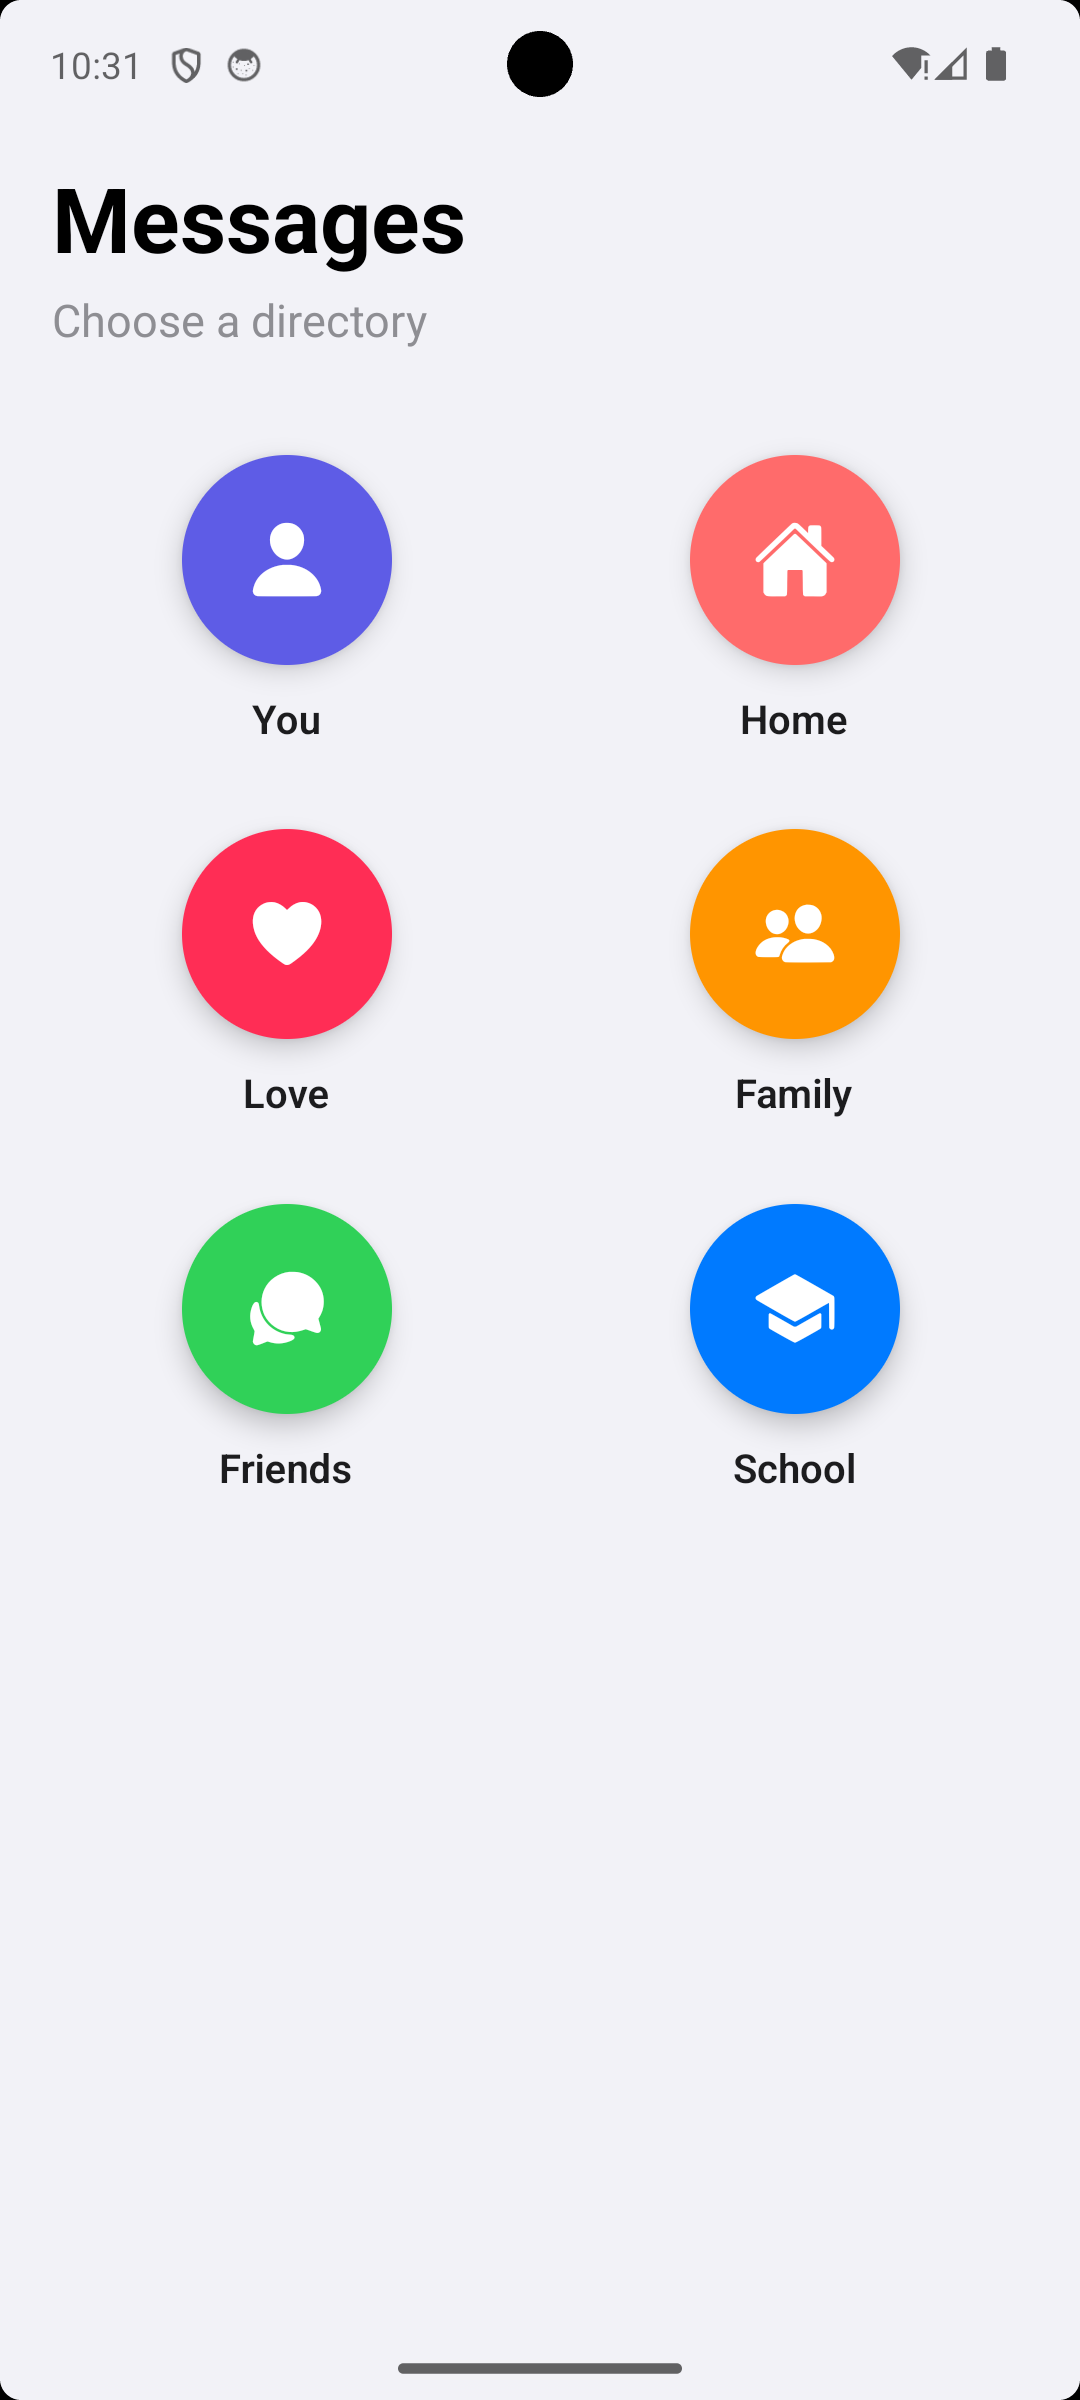
\includegraphics[width=0.45\textwidth]{Screenshot_20260501_103116.png}
    \caption{Home Screen --- Category Grid}
\end{figure}

\begin{figure}[H]
    \centering
    \begin{minipage}{0.45\textwidth}
        \centering
        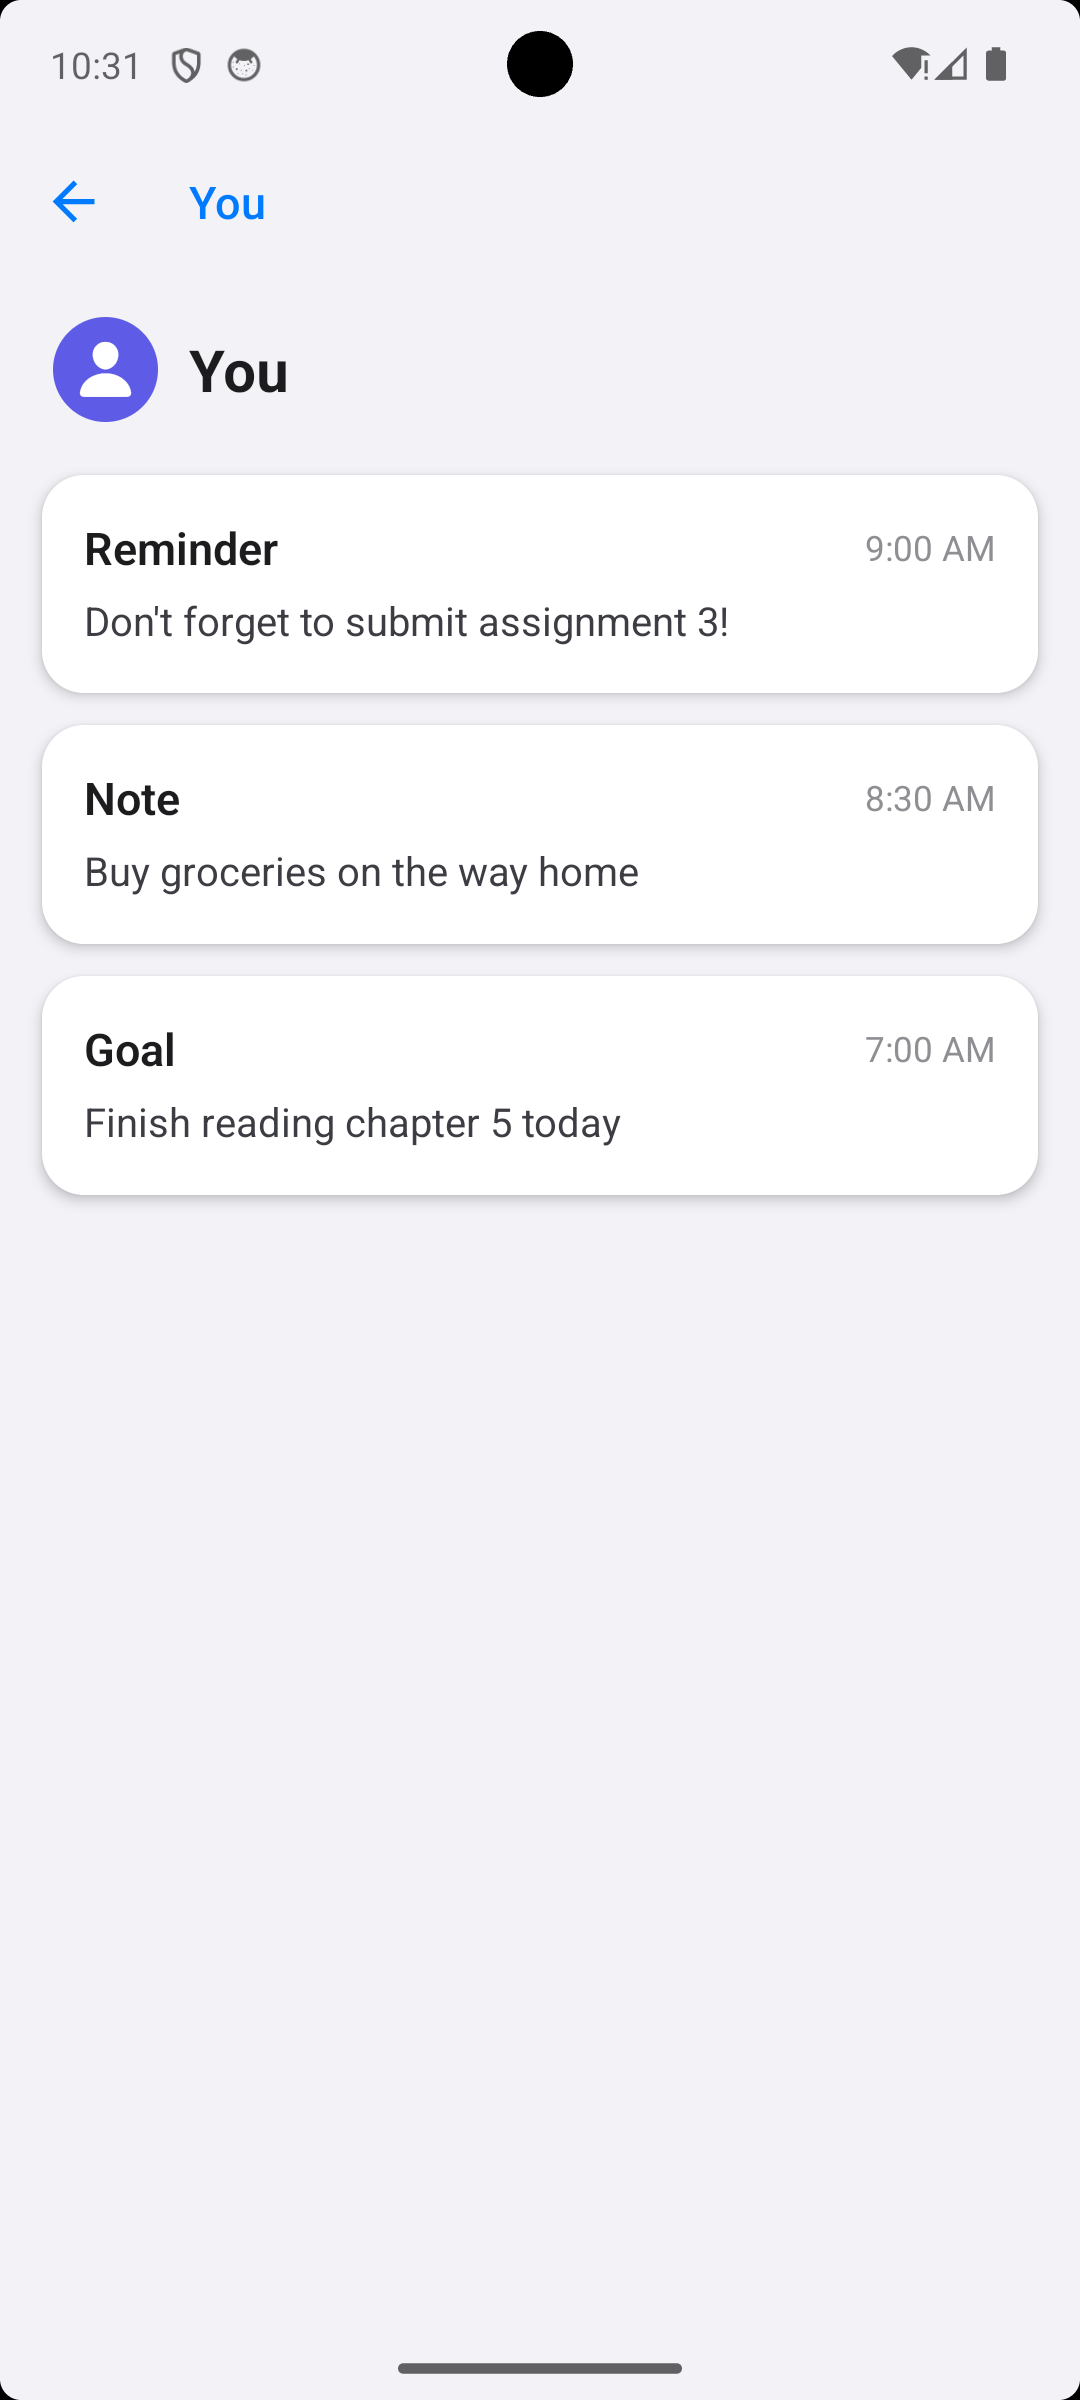
\includegraphics[width=\textwidth]{Screenshot_20260501_103140.png}
        \caption{You Messages}
    \end{minipage}
    \hfill
    \begin{minipage}{0.45\textwidth}
        \centering
        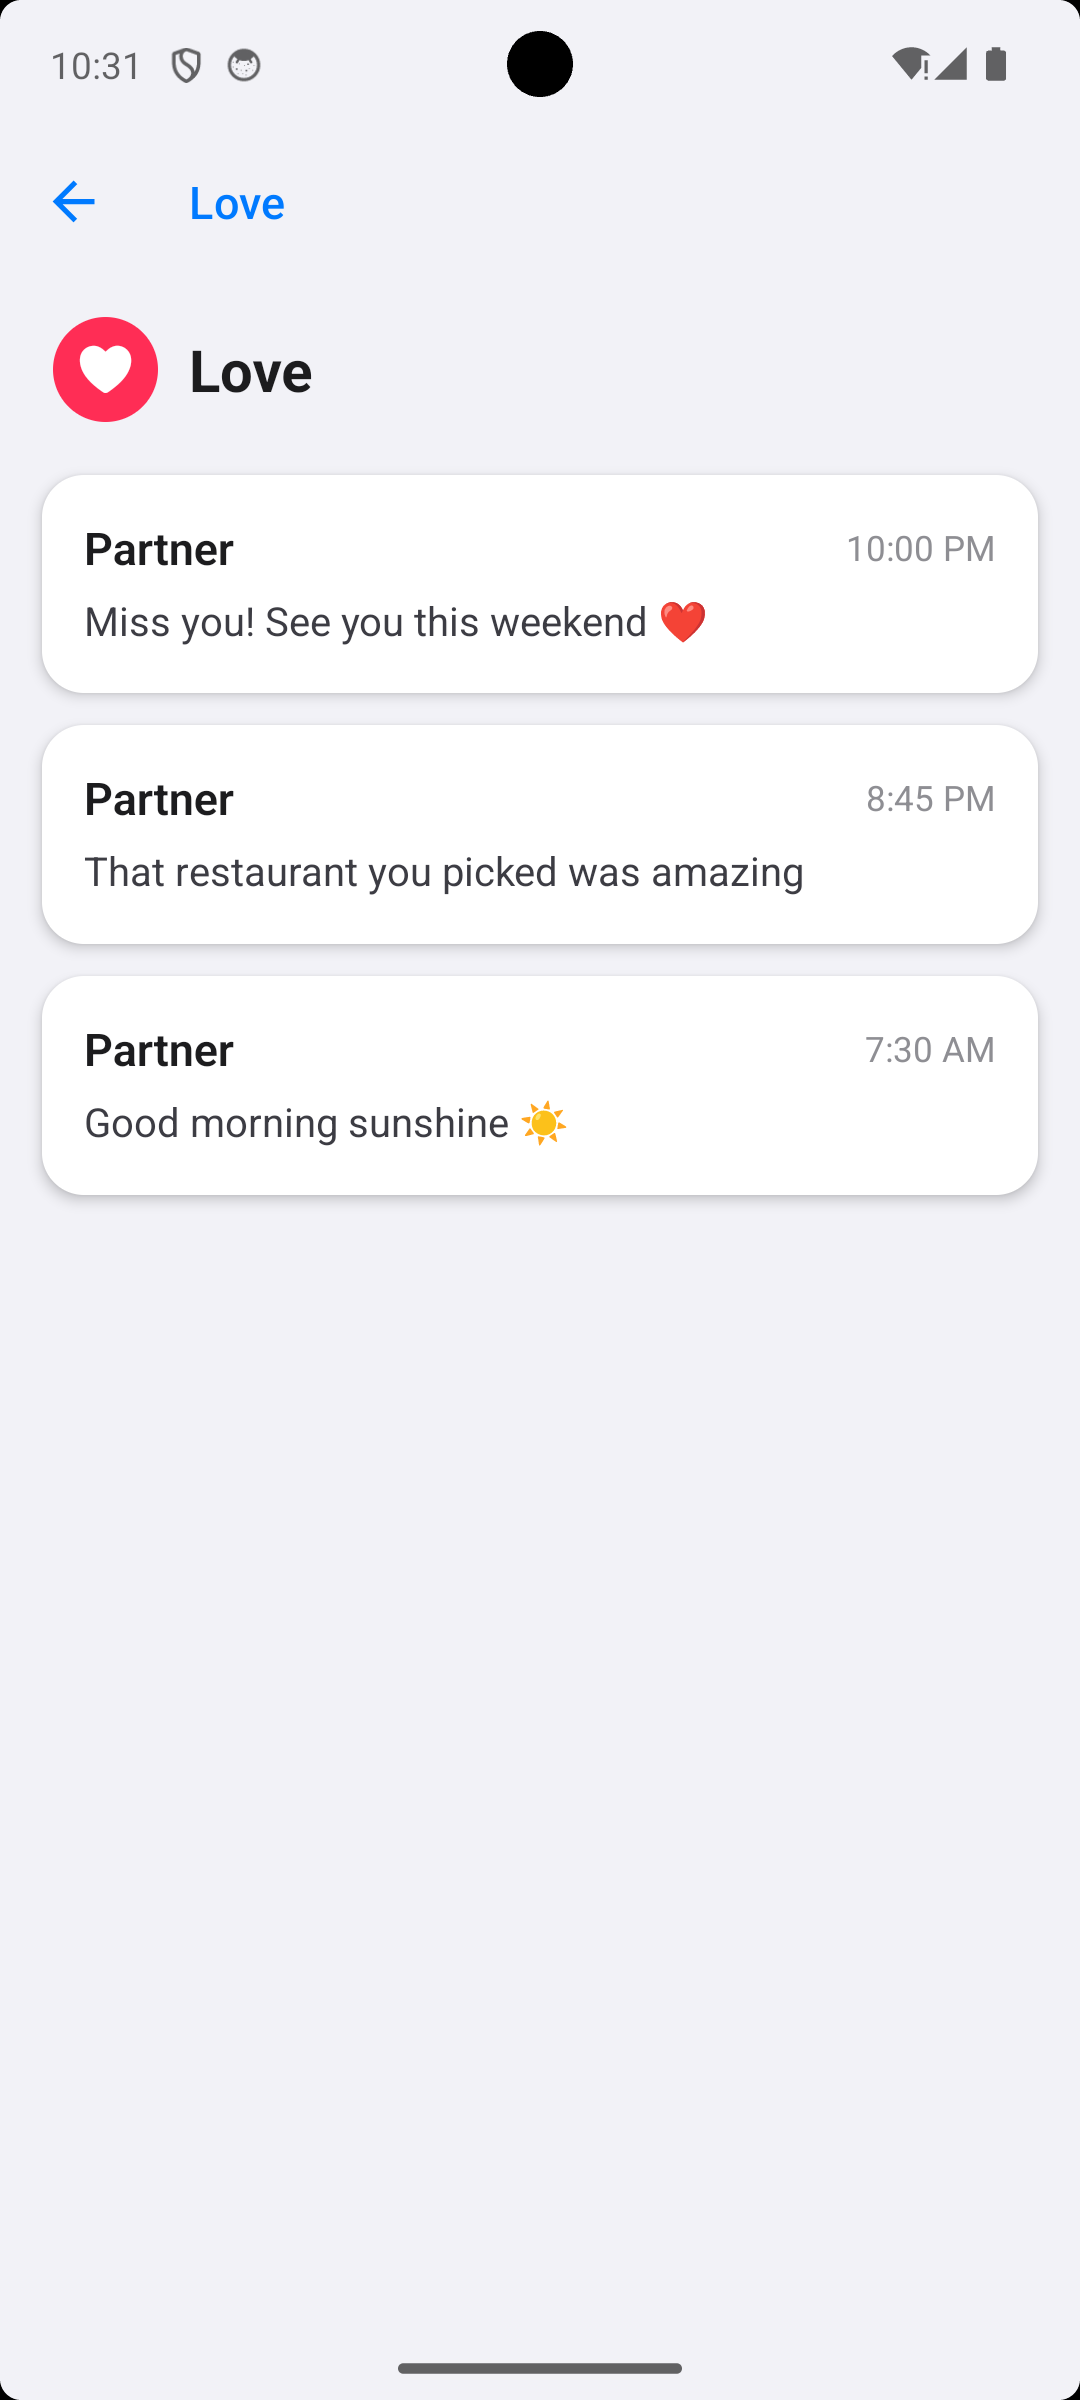
\includegraphics[width=\textwidth]{Screenshot_20260501_103153.png}
        \caption{Love Messages}
    \end{minipage}
\end{figure}

\begin{figure}[H]
    \centering
    \begin{minipage}{0.45\textwidth}
        \centering
        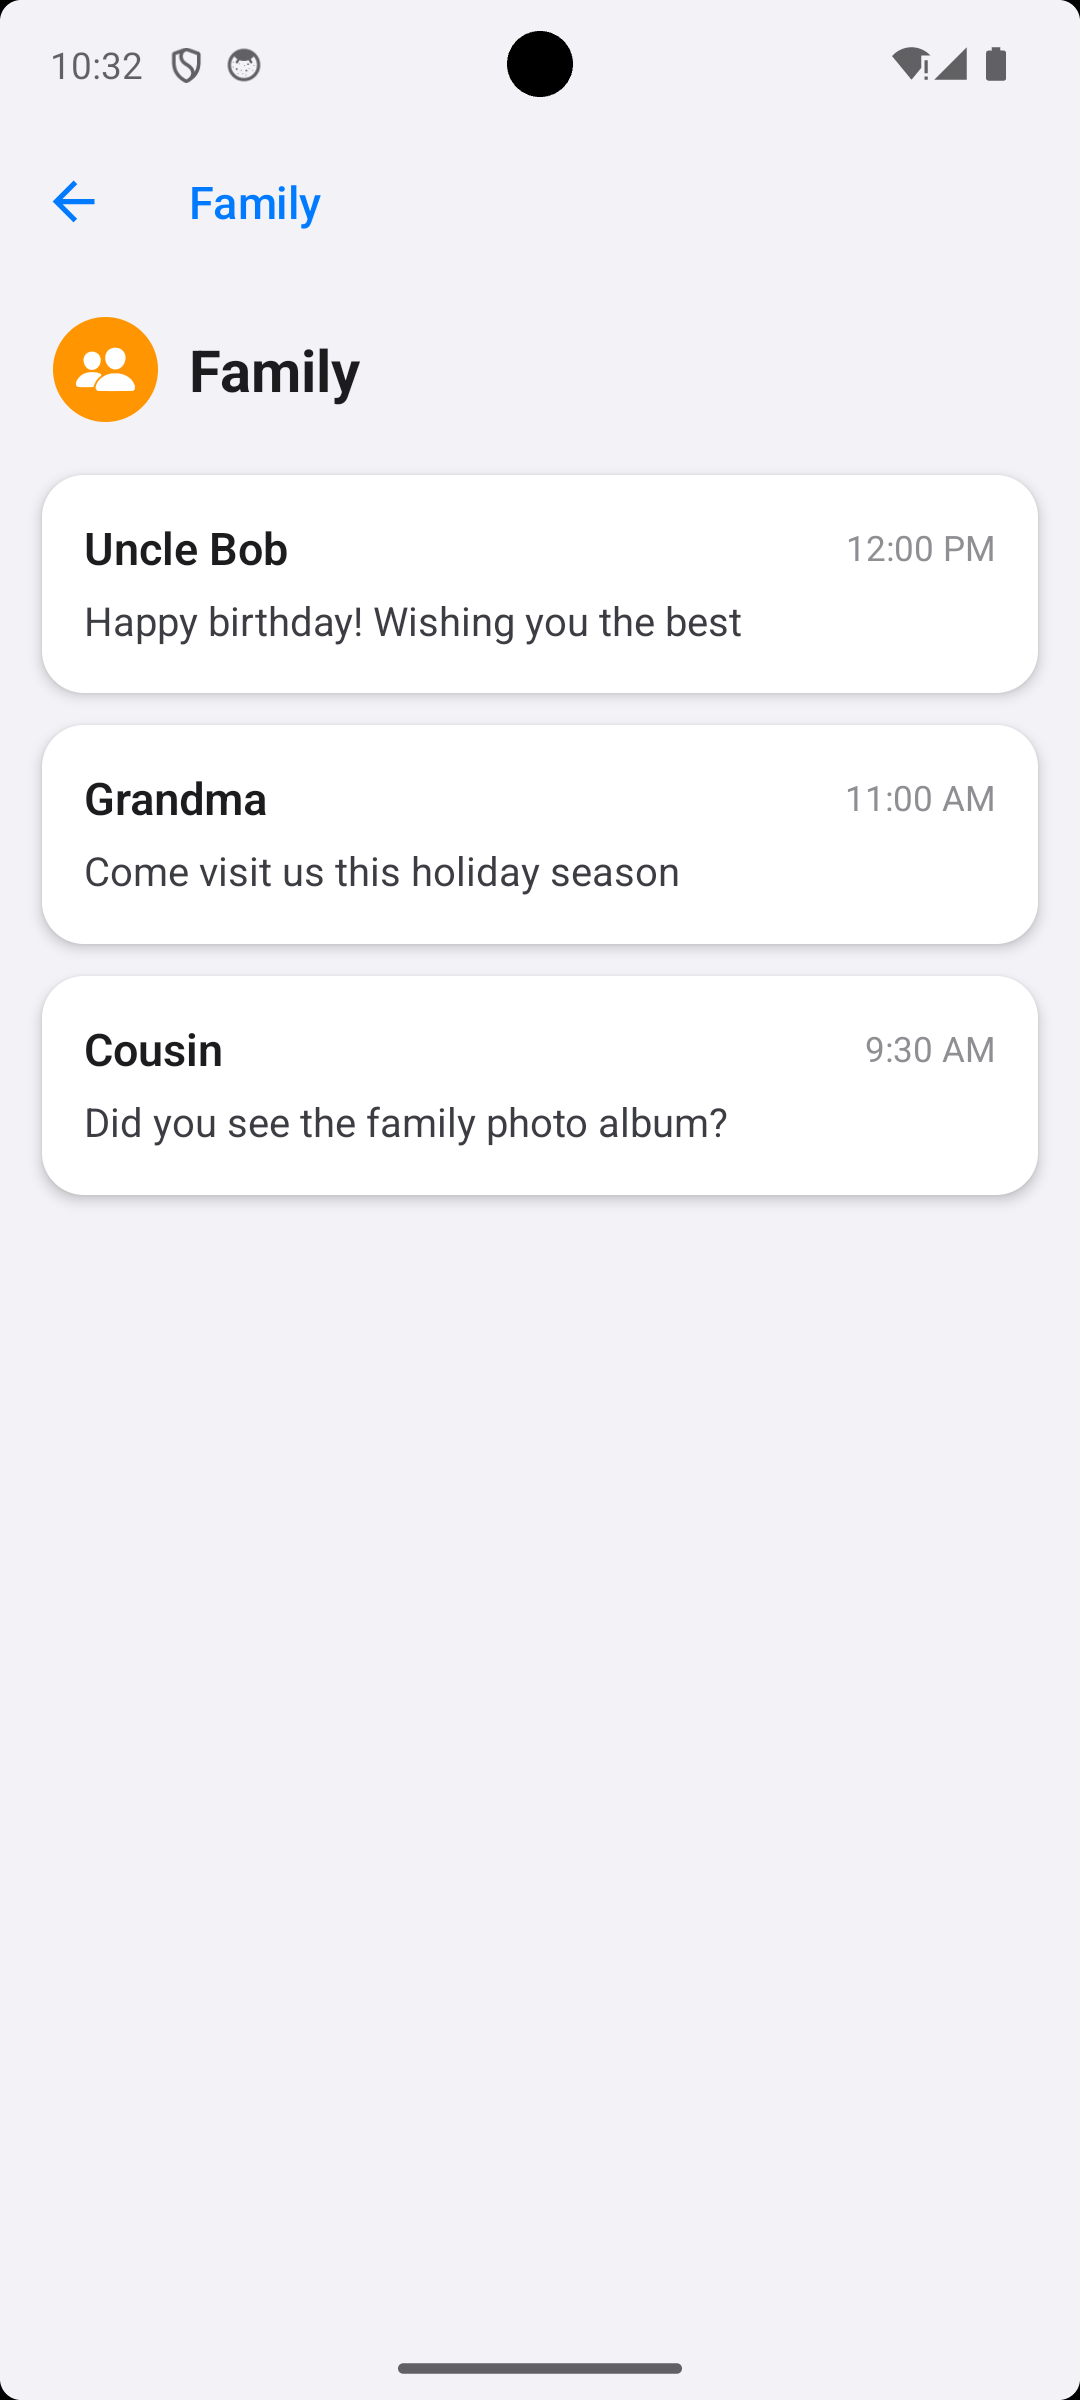
\includegraphics[width=\textwidth]{Screenshot_20260501_103200.png}
        \caption{Family Messages}
    \end{minipage}
    \hfill
    \begin{minipage}{0.45\textwidth}
        \centering
        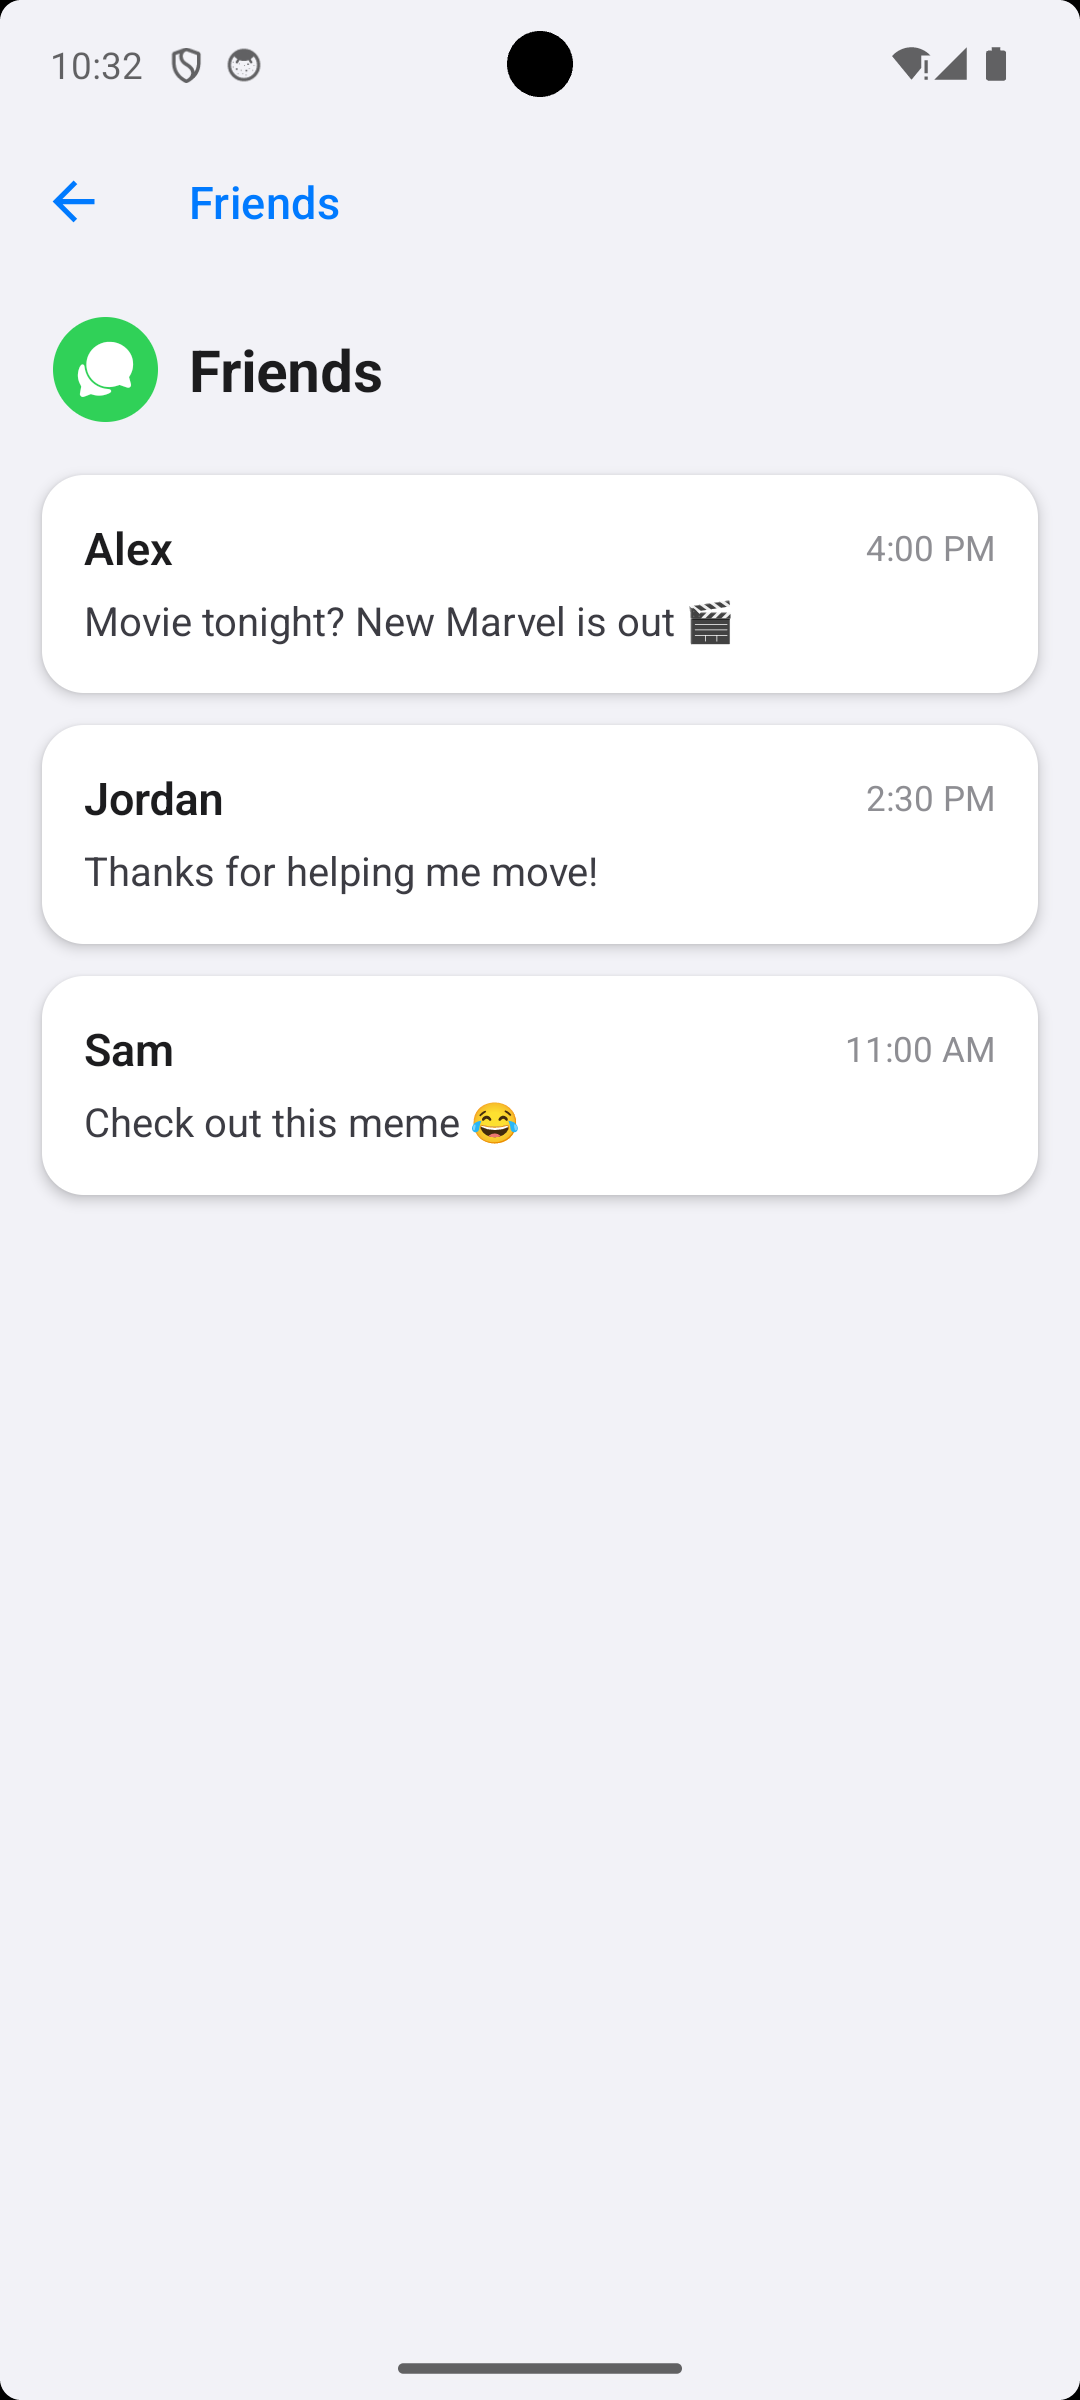
\includegraphics[width=\textwidth]{Screenshot_20260501_103206.png}
        \caption{Friends Messages}
    \end{minipage}
\end{figure}

\begin{figure}[H]
    \centering
    \begin{minipage}{0.45\textwidth}
        \centering
        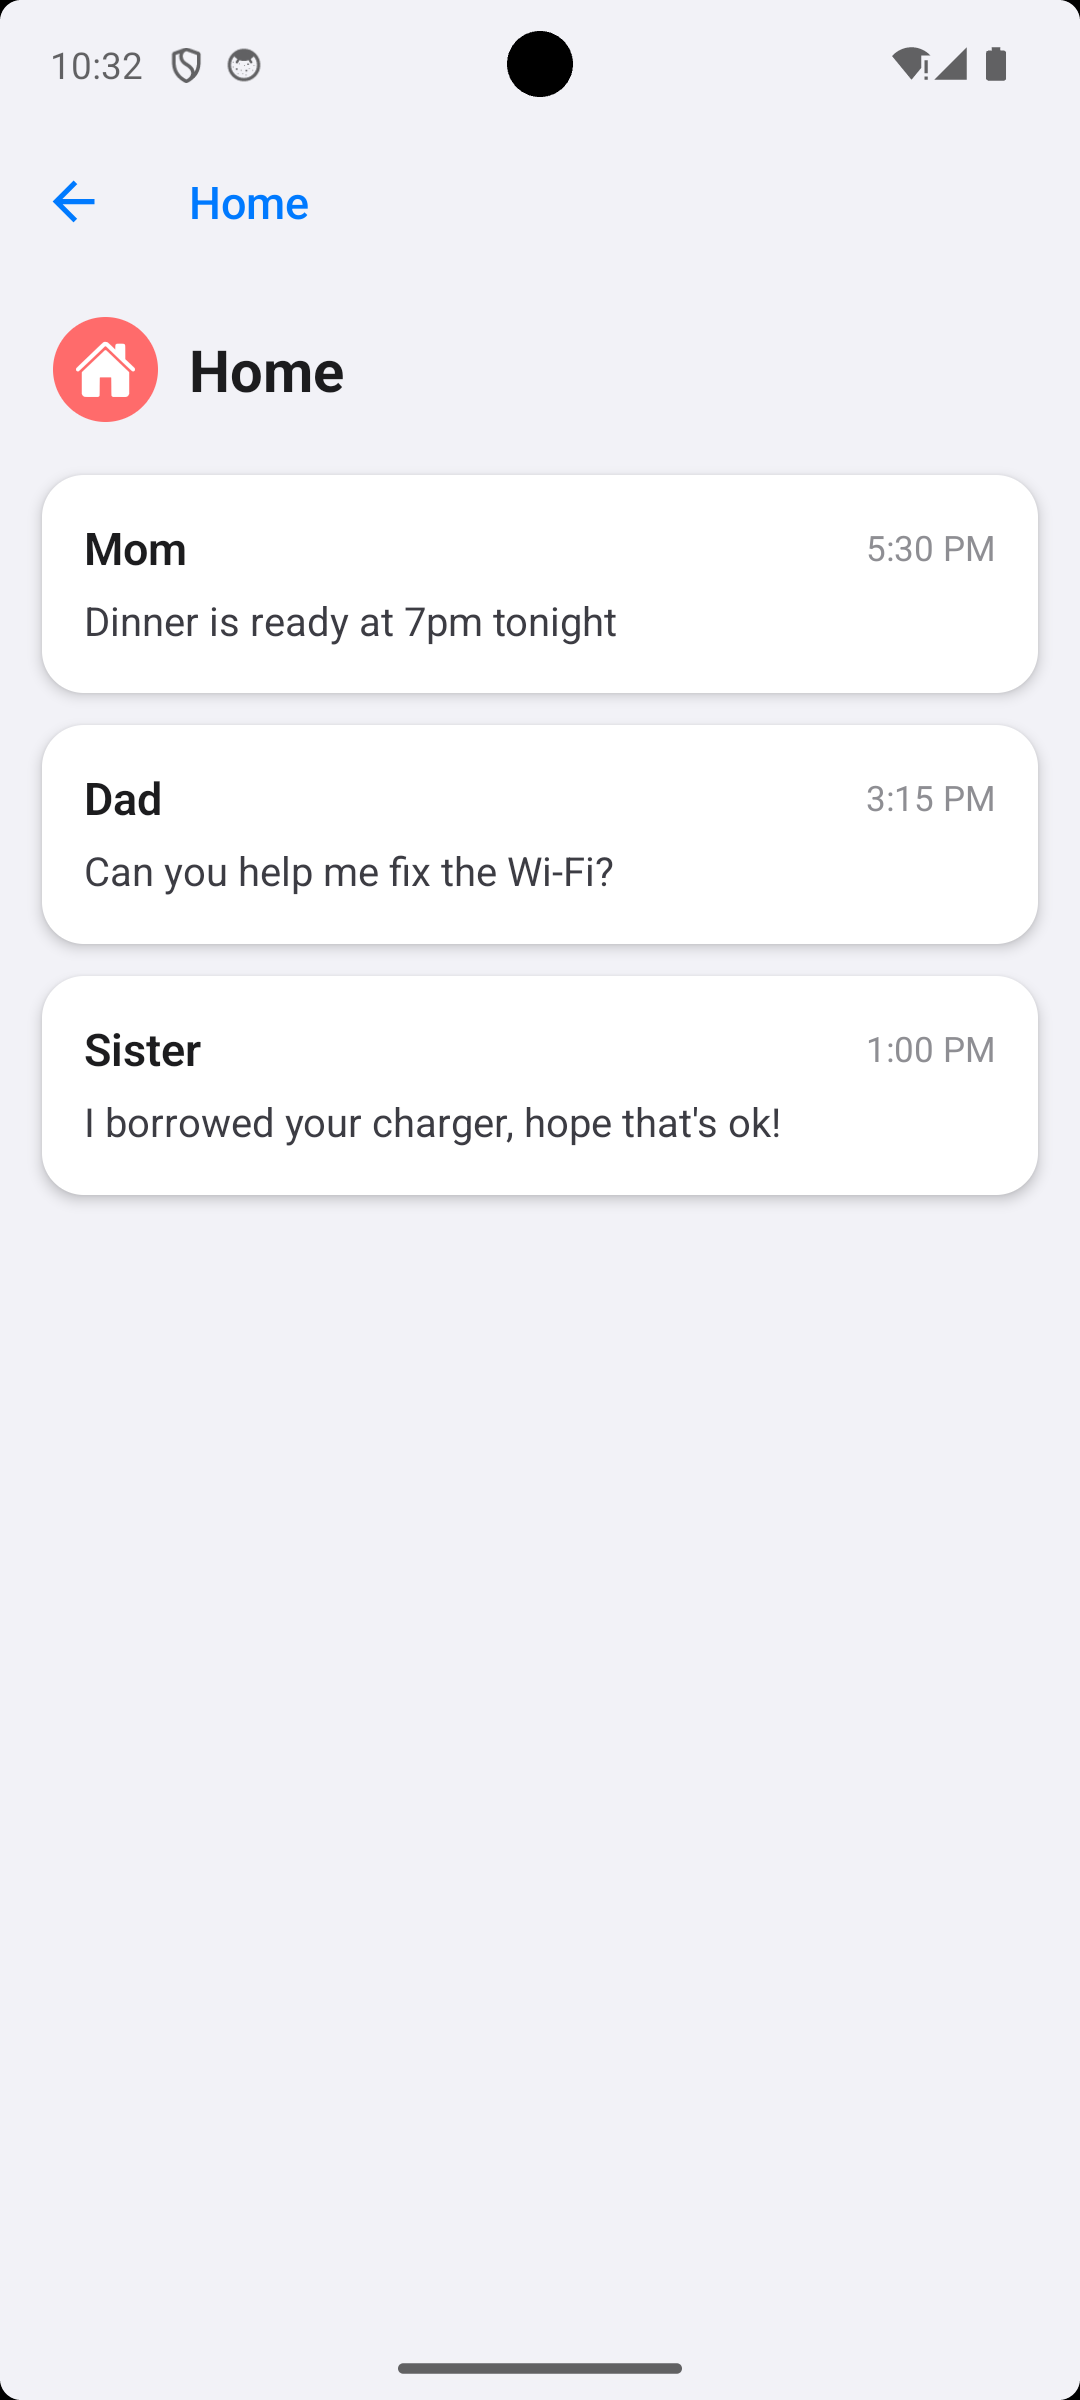
\includegraphics[width=\textwidth]{Screenshot_20260501_103212.png}
        \caption{Home Messages}
    \end{minipage}
    \hfill
    \begin{minipage}{0.45\textwidth}
        \centering
        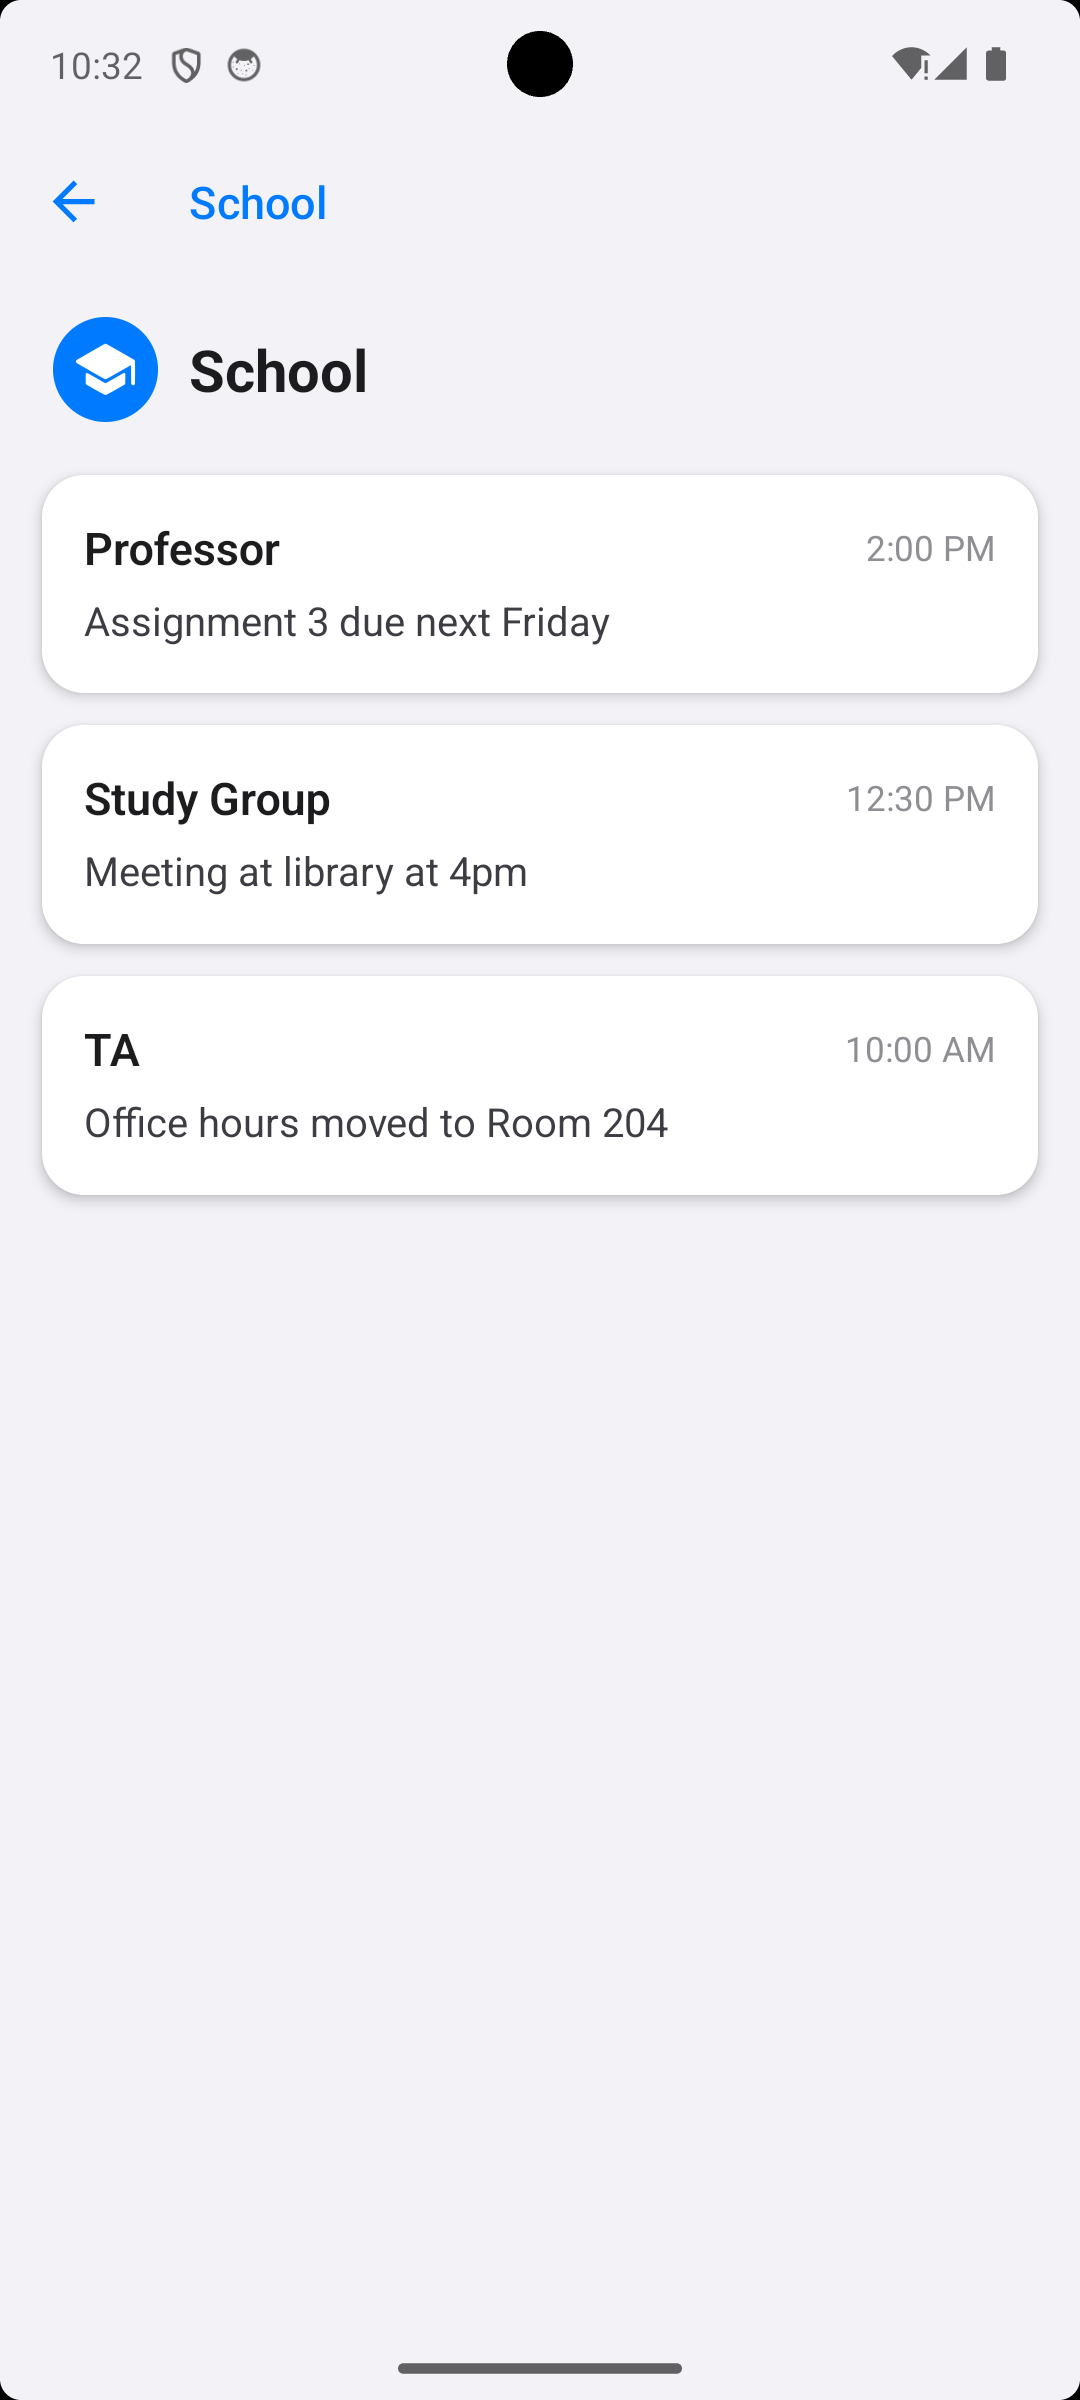
\includegraphics[width=\textwidth]{Screenshot_20260501_103220.png}
        \caption{School Messages}
    \end{minipage}
\end{figure}

\begin{figure}[H]
    \centering
    \begin{minipage}{0.45\textwidth}
        \centering
        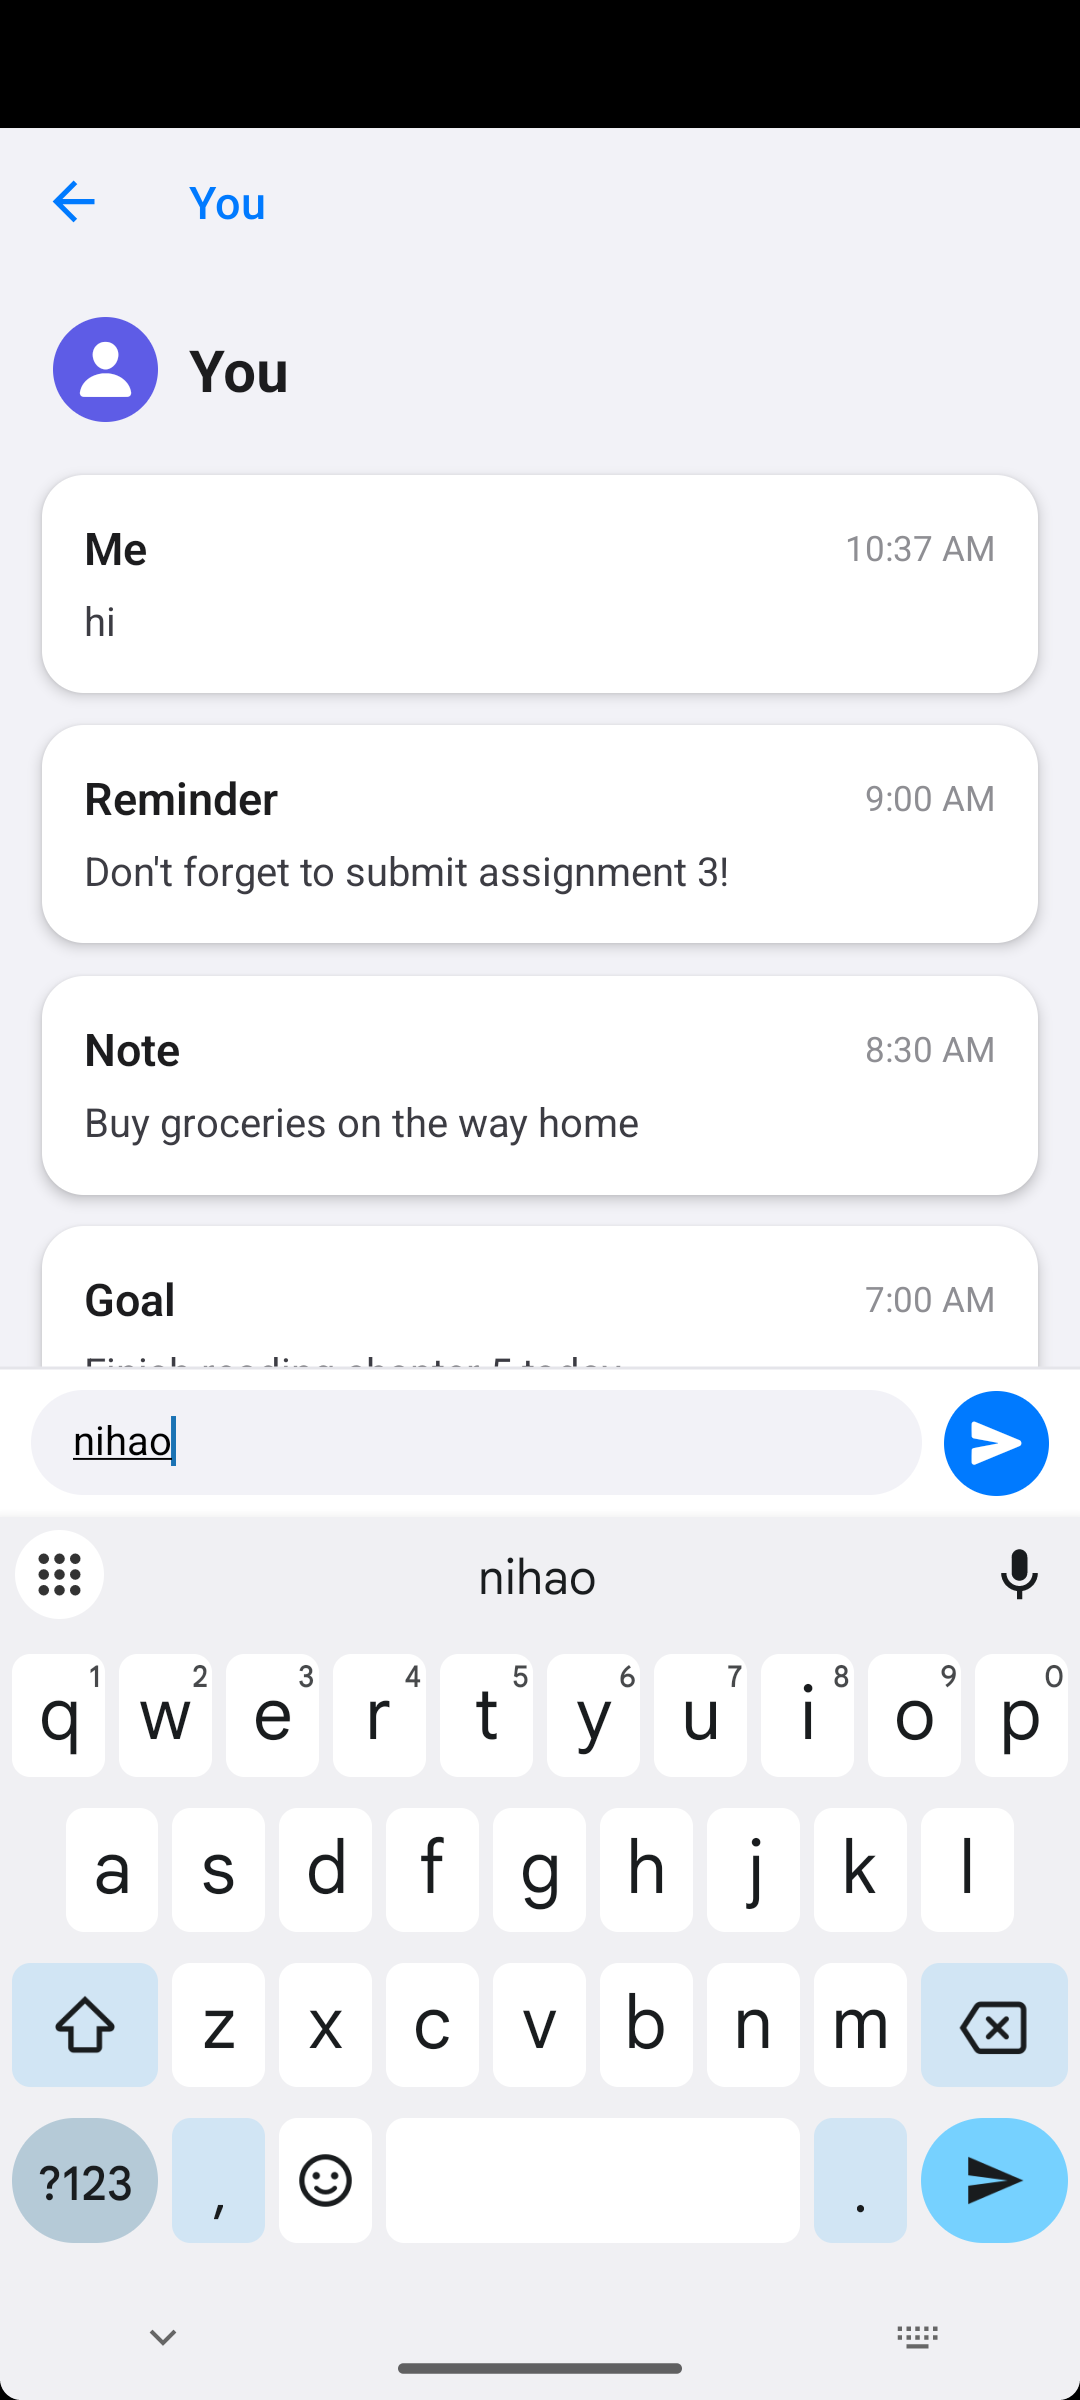
\includegraphics[width=\textwidth]{Screenshot_20260501_103748.png}
        \caption{Send Message}
    \end{minipage}
    \hfill
    \begin{minipage}{0.45\textwidth}
        \centering
        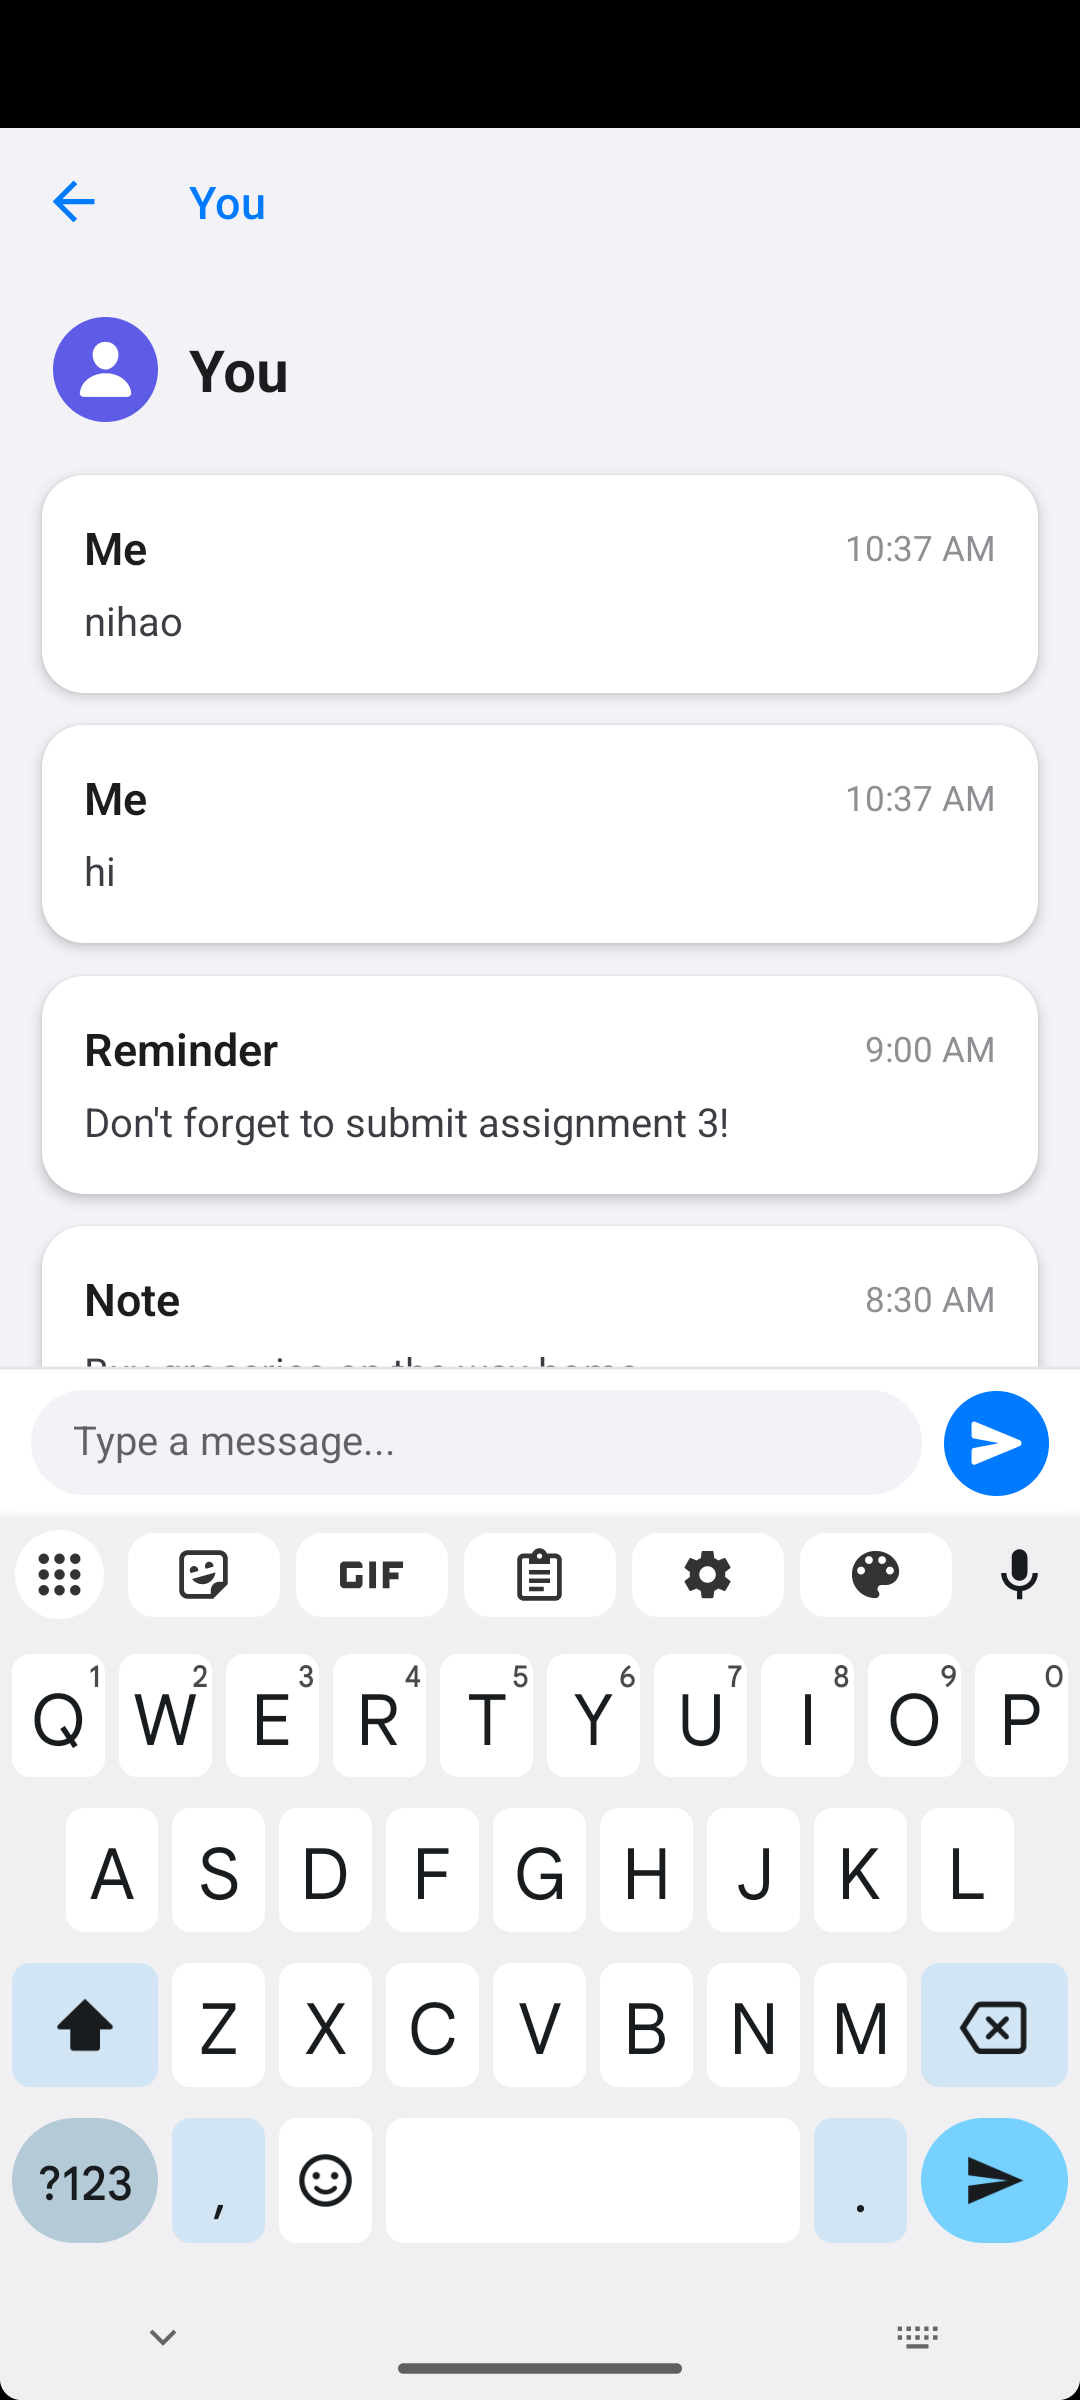
\includegraphics[width=\textwidth]{Screenshot_20260501_103753.png}
        \caption{Send Message Result}
    \end{minipage}
\end{figure}

\end{document}
